\section{Funktionsweise und Frequenzgang eines Integrators}
Bei diesem Versuch wird ein Integrator aufgebaut mittels des Operationsverstärker. Der Aufbau erfolgt nach der Abbildung \ref{fig:Versuch2/Schaltbild eines Integrators} in die Schaltung wird für R= 1 $k \Omega$ und C= 10 $nF$ genommen, welche vorher gemessen werden mittels eines Multimeters und die Fehler können als vernachlässigbar angesehen werden. Der Sweep-Modus wird im Funktionsgenerator ausgeschaltet sowie wird eine Frequenz von 1 $kHz$, eine Amplitude von 500 $mV$ und einen DC-Offset von 0 $V$ eingestellt. Mit dem Oszilloskop wird dann die Eingangsspannung $U_1$ und die Ausgangsspannung $U_2$ des Operationsverstärkers gemessen und werden die Bilder einer Rechteckspannung, einer Dreiecksspannung und einer Sinusspannung mit der integrierte Form, die über die Ausgangsspannung $U_2$ ausgegeben wird, gespeichert.   
\begin{figure}[H]
    \centering
    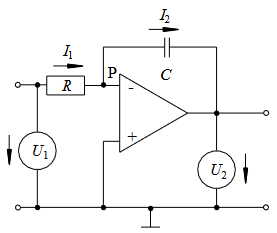
\includegraphics[width=0.4\textwidth]{2023-04-17 - V2 -Operationsverstärker/images/Funktionsweise und Grequenzgang eines Integrators Aufbau.png}
    \caption{Schaltbild eines Integrators entnommen aus \csite{script}
    \label{fig:Versuch2/Schaltbild eines Integrators}
\end{figure}
In der Abbildung \ref{fig:Versuch2/Darstellung einer Rechteckspannung und einer integrierten Dreiecksspannung} ist der Verlauf der Rechteckspannung, welche hier Gelb dargestellt wird und über den ersten Channel gemessen wird. Die über den zweiten Channel dargestellte Messung zeigt den intrigierenten Verlauf der von Channel 1. Sich bar wird dies, wenn man vom Triggerpunkt aus guckt, wo die Rechteckspannung positiv ist und die Dreieck ihren Höhepunkt hat und ab da an anfängt abzufallen und erst dann wieder anfängt zu steigen, wenn die Rechteckspannung ihren Tiefpunkt erreicht hat. 
\begin{figure}[H]
    \centering
    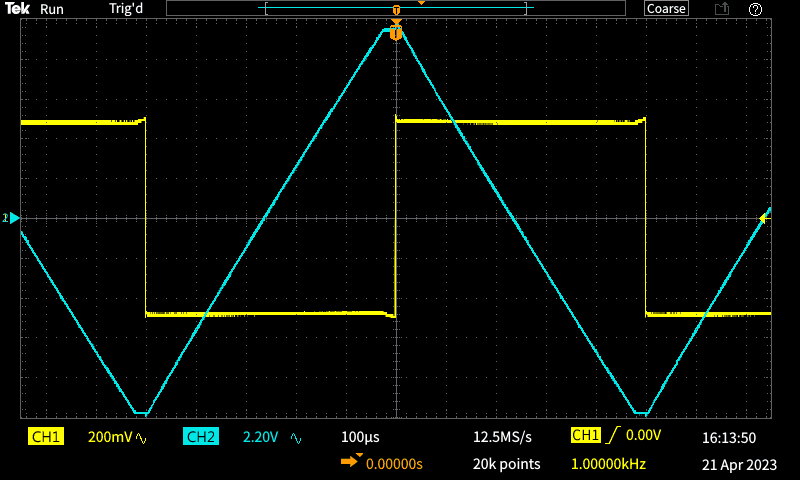
\includegraphics[width=0.75\textwidth]{TEK00000.PNG}
    \caption{Darstellung einer Rechteckspannung und einer integrierten Dreiecksspannung}
    \label{fig:Versuch2/Darstellung einer Rechteckspannung und einer integrierten Dreiecksspannung}
\end{figure}
\begin{figure}[H]
    \centering
    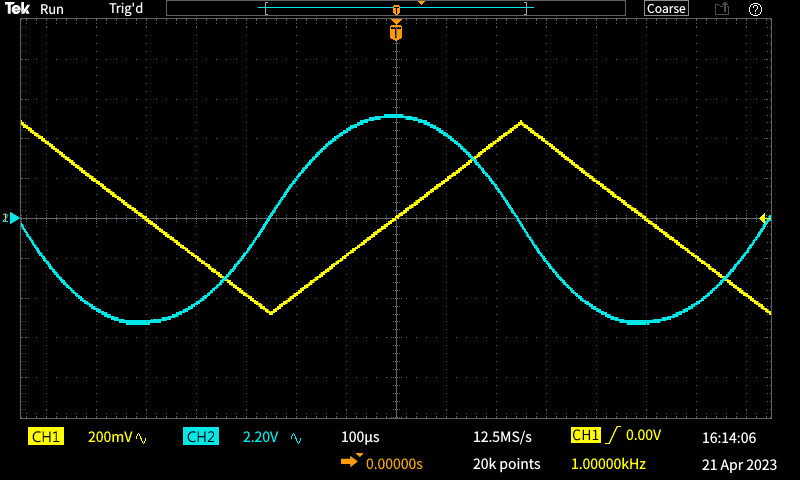
\includegraphics[width=0.75\textwidth]{TEK00001.PNG}
    \caption{Darstellung einer Dreieckspannung und einer integrierten Sinusförmgenspannung}
    \label{fig:Versuch2/Darstellung einer Dreieckspannung und einer integrierten Sinusförmigenspannung}
\end{figure}
\begin{figure}[H]
    \centering
    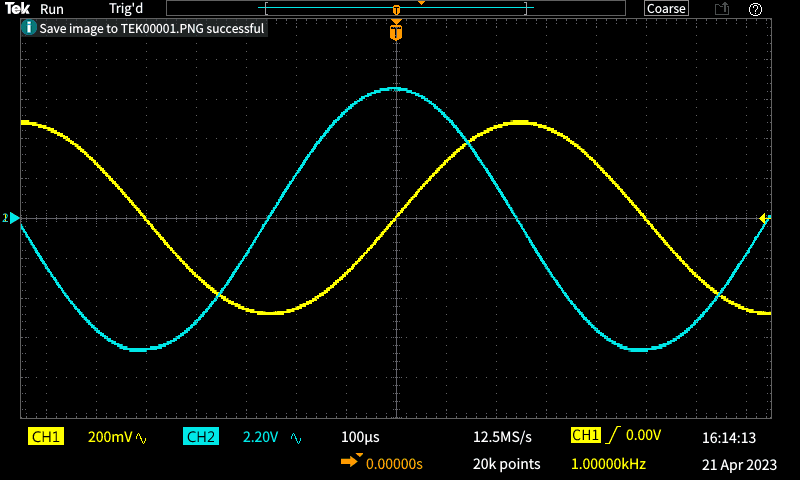
\includegraphics[width=0.75\textwidth]{TEK00002.PNG}
    \caption{Darstellung einer Sinusspannung und einer integrierten Cosinusförmigenspannung}
    \label{fig:Versuch2/Darstellung einer Sinusspannung und einer integrierten Cosinusförmigenspannung}
\end{figure}

